%%%%%%% This template was created by Brayden Lewis-Lord - s5182689 %%%%%%%%%
%%%%%%%%%%%%%%%%%%%%%%%%%%%%%%% 8/11/2023 %%%%%%%%%%%%%%%%%%%%%%%%%%%%%%%%%%

\documentclass[a4paper, twoside]{article}
\usepackage[backend=biber,style=ieee,sorting=none]{biblatex}
\usepackage{geometry}
\usepackage{amssymb}
\usepackage{subcaption}
\geometry{a4paper,total={170mm,250mm},left=20mm, top=20mm,}
\usepackage{enumerate}
\usepackage[shortlabels]{enumitem}
\usepackage{optidef}
\usepackage[normalem]{ulem}
\useunder{\uline}{\ul}{}
\addbibresource{mybibliography.bib}
\usepackage{datetime}
\usepackage{xcolor}
\usepackage{booktabs}
\newdateformat{monthyeardate}{
\monthname[\THEMONTH], \THEYEAR}
\date{\monthyeardate\today}
\usepackage{parskip}
\setlength{\parskip}{0.4em}
\DeclareMathOperator*{\argmin}{arg\,min}
\usepackage{commath}
\usepackage{tikz}
\usetikzlibrary{arrows.meta,positioning}
\usepackage{graphicx,caption}
\usepackage{amsmath}
\usepackage{multirow}
\usepackage{graphicx}
\usepackage[table]{xcolor}
\usepackage[utf8]{inputenc}
\usepackage{amsmath, amssymb}
\usepackage{geometry}
\usepackage{graphicx}
\usepackage{hyperref}
\usepackage{enumitem}
\usepackage{fancyhdr}
\usepackage{caption}
\usepackage{appendix}
\usepackage{float}
\usepackage{tikz}   % For drawing the factor graph (optional)
\DeclareMathOperator*{\argmax}{arg\,max}
\renewcommand{\thesubsubsection}{\alph{subsubsection}.}
\usepackage{listings}
\lstset{
    language=C++,
    basicstyle=\ttfamily\small,
    breaklines=true,
    showstringspaces=false
}
%%%%%%%%%%%%%%%%%%%%%%%%%%%%%%%%%%%%%%%%%%%%%%%%%%%%%%%%%%%%%%%%%%%%%%%%%%%%%%%%%%%%%
%%%%%%%%%%%%%%%%%%%%%%%%%%%   Enter Your info here    %%%%%%%%%%%%%%%%%%%%%%%%%%%%%%%

\author{Pablo Bustos, Jorge Calderón, Adrián Sánchez and José Manuel Torres-Domínguez, Jesús Martínez, Javier Ballesteros}
\def\coursecode{RL0024}
\def\assignname{RoboLab Technical Report Series}
\linespread{1.1}
\title{INSIGHT - Progress Report 1}

%%%%%%%%%%%%%%%%%%%%%%%%%%%%%%%%%%%%%%%%%%%%%%%%%%%%%%%%%%%%%%%%%%%%%%%%%%%%%%%%%%%%%%
\begin{document}
\input{title/title.tex}

\maketitle

\section{Introduction}

The \textbf{INSIGHT} project explores the concept of causal reasoning, an area that remains relatively unexplored in the field of robotics. We draw on C.S. Peirce's classic idea of abduction as \textit{inference to the best explanation} \cite{peirce1883theory}, and on J. Pearl's \textit{ladder of causality} \cite{pearl2018bookofwhy} to create and test hypotheses that explain the data from an unexpected experience. The project is designed around a single use case that is simple enough to let us focus on the theoretical needs, but can be easily extended into more complex human-robot and robot-environment interactions. 
In the proposed scenario, the robot Shadow follows its human supervisor, Anna, on a medicine delivery mission at a healthcare facility. Without noticing its presence, the robot hits a bump on the floor, and the medicine bottle falls off the tray. The robot detects that the bottle is gone and stops to draw Anna's attention to the new situation. In the short time that Anna stops, turns around and approaches the robot, Shadow has to build an explanation of the unexpected perceptive event. Also, using a resting period, it has to create a new agent to manage the new acquired concept \textit{bump}. This scenario is explained in more detail in \cite{bustos2025insight}. 
    
The project brings together three research groups in robotics and AI, using existing technology to accelerate development. This includes two mobile robots, Shadow \cite{torrejon_design_2024} and Morphia \cite{crucesSociallyAssistiveRobots2024}, designed as personal assistants that follow and carry objects for humans in indoor environments; and the CORTEX cognitive architecture for robotics, as described in  \cite{luis-pablo-cortex} and \cite{calderita_estevez_deep_2015}, which provides a robust development environment for exploring the cognitive abilities sought by the project.
    

\textbf{CORTEX} is an ongoing effort to develop a cognitive architecture for autonomous robots. It draws on the classical taxonomy of human memory systems---working, episodic, semantic, and procedural memory \cite{tulving1972episodic}\cite{squire2008memory}---and extends it with a long-term spatial memory commonly used in mobile robotics. Beyond memory modules, CORTEX also introduces \textit{agents}: processes that transfer and coordinate information across memories, typically by minimizing a task-specific loss function.
One agent manages an internal simulator that is used here to validate or discard alternative plausible causes before selecting one. It does that by replaying the content of the episodic memory extended with the new candidate factors that might have caused the anomaly.
 Figure \ref{fig:cortex_intro_image} shows an overall schema of the architecture, 
CORTEX has been described in several works before~\cite{proposal-latency-bustos,calderita_estevez_deep_2015}, as well as its application in different scenarios and use cases~\cite{react-navigation-cortex,luis-pablo-cortex,proposal-design-semantic}. The integration of an internal simulator has also been reported in~\cite{zapata_guessing_2024}. 
Here we focus on the elements redesigned and improved for this project, specifically the episodic memory, and the agents managing the robot, the room, the human, the medicine and the mission. 

Each memory in CORTEX is implemented as a distributed graph, where nodes encode entities, while edges encode the relationships between them, geometric or semantic, enabling relational reasoning and coherent information flow across the architecture. These graphs are implemented using Conflict-Free Replicated Data Types, CRDTs, as introduced in \cite{shapiro2011crdt}, over a reliable multicast protocol provided by a Data Distribution Service (DDS) implementation \cite{eprosima_fastdds_docs}. Taken together, this technology is offers a serverless, low-latency, high-throughput, eventually consistent access to the data by the intervening agents. The details can be found in  ~\cite{proposal-latency-bustos, garcia2021, dsr-icarsc2022}


\begin{figure}[h]
\centering
\includegraphics[width=0.9
\textwidth]{images/cortex.jpg}
\caption{The CORTEX architecture.}
\label{fig:cortex_intro_image}
\end{figure}

To achieve this, CORTEX is organised into five complementary memory modules:

\begin{itemize}
    \item \textbf{Working Memory (WM):} It stores the robot's current context. Its content is created and updated by the agents connected to it. Nodes in the WM represent entities detected in the environment or belonging to the robot, and edges capture relationships that express relative positions between elements or semantic constraints among them. We distinguish between structural and non-structural changes in WM, where structural changes involve adding or removing a node or an edge.
    
    \item \textbf{Episodic Memory (EM):} It stores what happens during mission execution by recording changes in Working Memory. The agent managing this memory detects the start and end of each robot mission and records its evolution by storing periodic keyframes and subsequent differential updates. Each mission is stored as a node in EM, and the agent provides methods to recover and query its contents.
    
    \item \textbf{Semantic Memory (SM):} It represents the robot's generic, not necessarily grounded, knowledge of the world, as a specialised version of the SOMA ontology \cite{bessler2021foundations}. The agent controlling SM is aware of structural changes in WM and validates them against the ontology using the Hermite inference engine. If the robot perceives a change in the world that cannot be logically explained, this agent triggers an explanation process that may end with learning a new concept.
    
    \item \textbf{Long-Term Spatial Memory (LTSM):} It maintains relationships between the different places and instances the robot traverses, enabling consistent, scalable, long-horizon spatial understanding. The agent managing LTSM is aware of WM evolution, removes previously visited places left behind, and loads stored places when the robot re-enters them. It can also plan routes through this representation.
    
    \item \textbf{Procedural Memory (PM):} It supports task decomposition by breaking complex missions (e.g., "bring me a soda") into simpler executable actions (e.g., "go to the fridge" and "open the fridge"), improving reuse and execution efficiency in future tasks. The agent managing PM uses a local large language model as a high-level task planner, and it is aware of WM state to provide, anticipate, and monitor task evolution.
\end{itemize}

All these memories are managed by a set of specialized agents that interact with the different modules, querying, updating, and synchronising information to sustain coherent cognitive behaviour during robot operation. % (see Figure~\ref{fig:cortex_intro_overview}).

\iffalse
\begin{figure}[h]
\centering
\resizebox{\textwidth}{!}{%
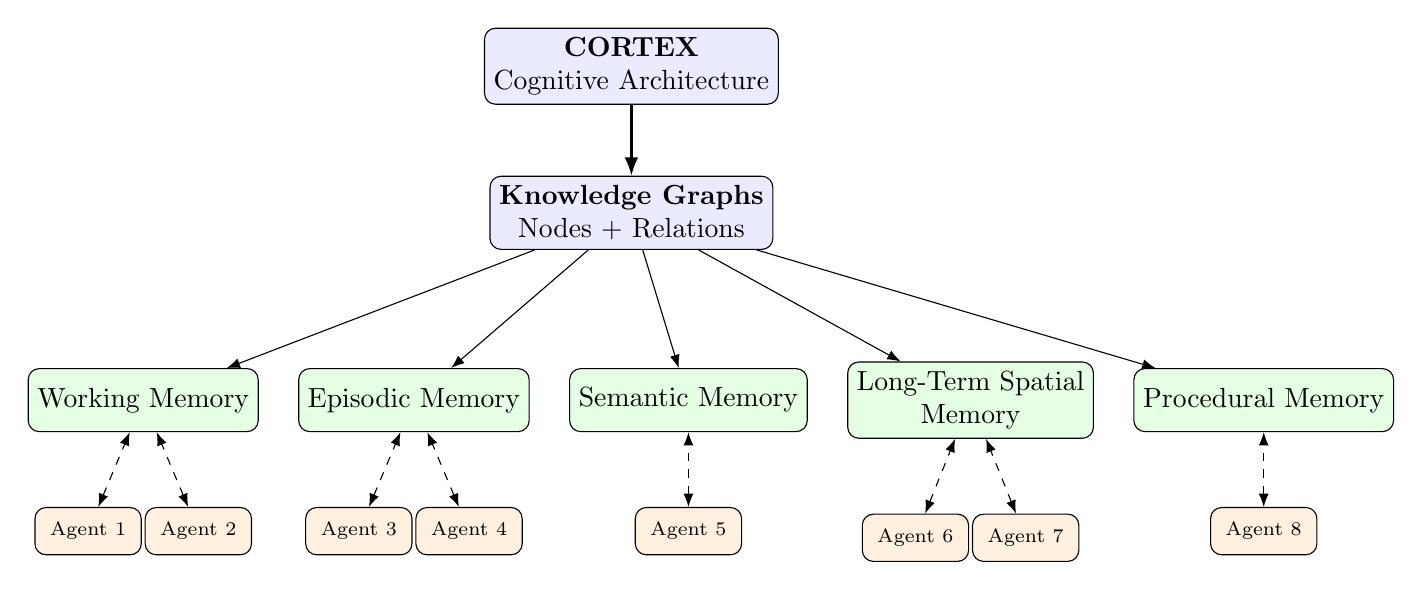
\begin{tikzpicture}[
    box/.style={draw, rounded corners, minimum width=2.9cm, minimum height=0.85cm, align=center, fill=blue!8},
    mem/.style={draw, rounded corners, minimum width=2.6cm, minimum height=0.8cm, align=center, fill=green!10},
    ag/.style={draw, rounded corners, minimum width=1.35cm, minimum height=0.6cm, align=center, fill=orange!12, font=\scriptsize},
    >=Latex,
    node distance=0.6cm
]

\node[box] (cortex) {\textbf{CORTEX}\\Cognitive Architecture};
\node[box, below=0.9cm of cortex] (kg) {\textbf{Knowledge Graphs}\\Nodes + Relations};

\node[mem, below=1.5cm of kg, xshift=-6.2cm] (wm) {Working Memory};
\node[mem, right=0.5cm of wm] (em) {Episodic Memory};
\node[mem, right=0.5cm of em] (sm) {Semantic Memory};
\node[mem, right=0.5cm of sm] (lsm) {Long-Term Spatial\\Memory};
\node[mem, right=0.5cm of lsm] (pm) {Procedural Memory};

\node[ag, below=0.95cm of wm, xshift=-0.7cm] (a1) {Agent 1};
\node[ag, below=0.95cm of wm, xshift=0.7cm] (a2) {Agent 2};

\node[ag, below=0.95cm of em, xshift=-0.7cm] (a3) {Agent 3};
\node[ag, below=0.95cm of em, xshift=0.7cm] (a4) {Agent 4};

\node[ag, below=0.95cm of sm, xshift=0cm] (a5) {Agent 5};

\node[ag, below=0.95cm of lsm, xshift=-0.7cm] (a6) {Agent 6};
\node[ag, below=0.95cm of lsm, xshift=0.7cm] (a7) {Agent 7};

\node[ag, below=0.95cm of pm, xshift=0cm] (a8) {Agent 8};

\draw[->, thick] (cortex) -- (kg);
\draw[->] (kg) -- (wm);
\draw[->] (kg) -- (em);
\draw[->] (kg) -- (sm);
\draw[->] (kg) -- (lsm);
\draw[->] (kg) -- (pm);

\draw[<->, dashed] (a1) -- (wm);
\draw[<->, dashed] (a2) -- (wm);

\draw[<->, dashed] (a3) -- (em);
\draw[<->, dashed] (a4) -- (em);

\draw[<->, dashed] (a5) -- (sm);

\draw[<->, dashed] (a6) -- (lsm);
\draw[<->, dashed] (a7) -- (lsm);

\draw[<->, dashed] (a8) -- (pm);

\end{tikzpicture}
}
\caption{Conceptual overview of CORTEX.}
\label{fig:cortex_intro_overview}
\end{figure}
\fi


\subsection{Progress}

The current Technical Report focuses primarily on the agents operating over \textbf{Working Memory}, \textbf{Episodic Memory} and \textbf{Semantic Memory}. At the current stage, concept agents do not yet perform real-world perception. Instead, they operate using object poses provided by the Webots simulator, which is currently treated as the reference "real" world for integration and testing.

% TODO: add a screencapture of the webots scenario

The agents involved in this report have different functions in the architecture. The \texttt{concept-X} agents manage the life-cycle of their concept instances detected in the environment, which include the robot itself, the human and the bottle carried by the robot. There is also an agent that controls the flow of information into and from the episodic memory, another for the semantic memory, an agent that controls the overall mission and and agent that manages an internal simulator used here for constrastive evaluation of plausible causes.

\begin{itemize}
    \item \texttt{concept\_person} [WM]: updates the target-person internal model in real time.
    \item \texttt{concept\_bottle} [WM]: updates the bottle internal models in real time.
    \item \texttt{concept\_robot} [WM]: updates robot internal state, controls robot motion to follow the selected mission target and publishes sensor measurements to Working Memory.
    \item \texttt{inner\_simulator} [WM, EM]: runs an internal simulation of the robot in its environment. The agent can run in synchronous mode, where the environment is recreated as perceived by the robot, or in evaluation mode, where it detaches from reality and replays stored experiences that can be modified with hypothetical variations.
    In synchronous mode the agent can raise alerts when significant mismatches are detected, providing a measure of normality.
    \item \texttt{mission\_controller} [WM]: manages target selection, mission start conditions, and mission completion state.
    \item \texttt{episodic\_memory\_agent} [WM, EM]: records Working Memory changes and publishes the consolidated mission trace after mission completion.
    \item \texttt{semantic\_memory\_agent} [WM, SM]: monitors structural changes in WM, validates them with the running ontology and triggers alerts when a change cannot be explained by its logic model. It searches for plaussible causes and proposes contrastive tests to be made by the internal simulator.
    
\end{itemize}


\section{Episodic Memory}

\subsection{Motivation}

Robots that operate for long periods in dynamic environments need more than an instantaneous world model: they also need a memory of \emph{what happened}, \emph{when it happened}, and \emph{under which context}. From a cognitive perspective, this aligns with the distinction between semantic and episodic memory introduced by Tulving, where episodic memory preserves temporally situated experiences rather than decontextualized facts \cite{tulving1972episodic,tulving1983elements}. In robotics, this distinction is especially relevant because many failures are not attributable to a single snapshot but to a sequence of events, actions, and interactions that unfold over time \cite{pugach2016episodic,dautenhahn1998episodic}. Episodic memory therefore provides temporal continuity by storing mission-relevant state transitions, actions, and observations as structured traces, enabling post-mission analysis, diagnosis, and explanation when an unexpected outcome cannot be inferred from the current state alone. In INSIGHT, these traces also support counterfactual reasoning through the internal simulator: past episodes can be replayed and contrasted with hypothetical alternatives to rank plausible causes and guide future decisions.

\subsection{Overall approach}
 The episodic memory (EM) in CORTEX is managed by a dual-connetion agent that has access to both the Working Memory and the EM. Its main role is to observe changes in the WM and log them to the EM. The main organisation unit is the \textit{mission}, understood as the time lapse between the start of a new task and its completion, or timeout. During that period, all structural and property derived changes not explicitily blacklisted are stored in a compact data structure in memory, called \textit{epoch}. As an epoch grows in size or when the mission has finished, it is stored in disk. The EM stores the current mission and the list of completed missions with some additional metadata used for retrieval.

% image of WW and EM being managed by the agent

% Detailed description of the differential encoding

\section{Internal Simulation}

\subsection{Motivation}

A service robot operating in unstructured environments will inevitably face situations that its exteroceptive sensors cannot fully explain: an unnoticed bump on the floor, a wheel that begins to slip, or a subtle mechanical degradation that manifests only through its dynamic response. The goal of the INSIGHT project is to detect these perceptual anomalies and transform them first into causal explanations and later into new actionable concepts.
A first step in this process is to detect latent failures that leave no direct visual or geometric trace. To this end, CORTEX includes an \emph{inner simulator} agent. One of its roles is to maintain a physics-based correlate of the real robot and detect discrepancies between expected and observed behaviour. These discrepancies are evaluated by other agents to determine whether the event is logically acceptable. If not, those agents generate a set of plausible causes that are evaluated through recreations of the event. These replays are augmented with candidate causes and tested against data stored in episodic memory. The overall process is contrastive: it discards improbable options and selects the best possible outcome under the available resources.

\subsection{Overall approach}

The inner simulator follows a \emph{hypothesise-and-test} strategy.
%% TODO: this won't exist on the near future. REDO!
In its online mode, the agent maintains a PyBullet scene containing the robot and relevant objects and publishes a synthetic IMU node (accelerometer and gyroscope) into the DSR graph.
The synthetic IMU is intended to be contrasted with the real IMU stream, while the full real history used for diagnosis is retrieved from episodic memory once an anomaly is flagged.

Problem detection is currently triggered externally by a dedicated request node in the DSR graph (e.g., a node whose name starts with \texttt{Search Problem Cause} and whose \texttt{status} attribute is set to \texttt{running}).
When this request is observed, the agent builds a \texttt{SimulationScene} descriptor (JSON) containing the scene parameters and a replay control profile, and enters the \emph{cause-evaluation} phase.
In this phase the agent loads the candidate causes from a JSON catalogue, spawns one independent \texttt{CausesSimulator} subprocess per cause, collects the simulated IMU traces, and ranks them against the real IMU trace retrieved from episodic memory.
The best-scoring runs, together with their sampled parameters, are stored in an output JSON report that can be attached to the mission log.

\subsection{Internal simulation}

The CORTEX internal simulator is built on top of the PyBullet physics engine.
At start-up, the agent loads URDF models for the ground plane, the robot chassis (a four-wheeled differential-drive platform), and any static objects present in the scene.
A task-relevant carried object (the medicine bottle) is also instantiated so that its pose can be monitored during replay.
A fixed time-step of $\frac{1}{62}$~s is configured to keep the simulation deterministic and reproducible.

At every simulation step the agent can convert commanded robot velocities into individual wheel angular velocities through a standard differential-drive kinematic model and apply them to the simulated wheels via motor velocity-control commands.
In the replay-based evaluation stage, the forward speed command is not read live but from a time-indexed profile stored in the \texttt{SimulationScene} descriptor (typically reconstructed from episodic memory as a piecewise-constant history of \texttt{robot\_ref\_adv\_speed}).

An IMU sensor model attached to the robot body produces accelerometer and gyroscope readings at every step by finite-difference differentiation of the base velocity, rotation into the IMU frame, and low-pass filtering to reduce numerical noise:

\begin{equation}
    \tilde{a} \;=\; R_{W}^{\,\mathrm{IMU}}\, a,
\end{equation}

\noindent where $R_{W}^{\,\mathrm{IMU}}$ is the rotation matrix from the world frame to the IMU frame, and $a$ is the linear acceleration computed by finite differences on the body velocity. In the current implementation, bias and white-noise terms are disabled and the same low-pass filter coefficient is also applied to the gyroscope signal.
The resulting synthetic IMU node (\texttt{imu\_sintetic}) is inserted into the DSR graph so that other agents can monitor it alongside the real sensor node.

\subsection{Problem detection and scene capture}

For diagnosis, the agent retrieves a timestamped real IMU trace from episodic memory, which has been recorded during mission execution.
Problem detection is triggered externally by a dedicated request node in the DSR graph.
At that moment, the agent captures the simulation-scene context---gravity, the initial robot and bottle poses, the problem pose, the mission duration, a time-indexed forward-speed profile, and a configurable number of repetitions---and serialises it into a structured descriptor (\texttt{SimulationScene}) that will be consumed by the cause-evaluation subprocesses.

In the current prototype, both the simulation-scene descriptor and the list of candidate causes are represented as JSON files (\texttt{src/sim\_scene.json} and \texttt{src/causes.json}).
This separation of concerns allows the cause-definition vocabulary to evolve independently from the simulation engine: new types of disturbances can be introduced by updating the cause catalogue without modifying any inner-simulator code.

\subsection{Cause evaluation}

The core of the diagnostic reasoning resides in the cause-evaluation pipeline.
Each candidate cause is described by a JSON payload that specifies a cause type and its associated parameters.
For example, a \emph{bump} cause carries the path to a URDF obstacle model together with the spatial region where the obstacle might have appeared, while a \emph{wheel} cause specifies which wheel is hypothesised to have failed and, optionally, a time-distribution parameter controlling when the failure occurs during the run.

\subsubsection{Parallel simulation}

For every cause in the catalogue, the agent spawns an independent child process that instantiates its own PyBullet environment.
Communication between parent and child relies on Unix pipes: the parent creates a pipe pair, passes the write-end file descriptor to the child, and reads the result from the read end once the child terminates.
This architecture avoids shared-memory complexity and allows each simulation to run in complete isolation, which is particularly important because PyBullet maintains global state that cannot be safely shared across threads.

Each child process performs the following steps:

\begin{enumerate}
    \item \textbf{Scene initialisation.} The simulation-scene descriptor is loaded and applied: gravity is set, the robot and bottle are placed at their recorded initial poses, and the forward-speed replay profile is configured.
    \item \textbf{Cause validation.} The JSON cause payload is validated against a dynamically-built Pydantic discriminated union that encompasses all known cause types. At import time, the simulator scans the cause-implementations directory, discovers every concrete subclass of the abstract \texttt{Cause} interface, and assembles a union type keyed on the \texttt{name} literal of each subclass. This mechanism makes the system fully extensible: dropping a new Python file into the implementations folder is sufficient for it to be recognised automatically.
    \item \textbf{Repeated simulation.} The cause is executed for the configured number of repetitions. Before each run the cause's \texttt{apply} hook prepares the scene---for instance, by spawning an obstacle at a randomly sampled position within the specified region. During each simulation step the cause's \texttt{apply\_compute} hook injects time-dependent behaviour---for instance, disabling a wheel motor once the elapsed time exceeds a random threshold. The simulated IMU records accelerometer and gyroscope readings at every step.
    \item \textbf{Result transmission.} After all repetitions, the collected IMU histories, together with the specific random-parameter instantiations used in each run and auxiliary state such as the final bottle pose, are serialised as JSON and written to the pipe for the parent to consume.
\end{enumerate}

\subsubsection{Trace comparison and ranking}

Once all child processes have finished and the parent has collected their outputs, the agent compares each simulated IMU trace against the real recording captured during the mission.
For every simulated frame, the closest real frame in time is identified and the Euclidean distance between the two accelerometer vectors and the two gyroscope vectors is computed.

If $(a_i,\omega_i,t_i)$ denotes a simulated sample and $(\hat a_j,\hat\omega_j,\hat t_j)$ a real sample, the closest-match index is $j(i)=\argmin_j\,|t_i-\hat t_j|$ and the per-frame distance is

\begin{equation}
    d_i \,=\, \frac{\lVert a_i-\hat a_{j(i)}\rVert_2 + \lVert \omega_i-\hat\omega_{j(i)}\rVert_2}{2}.
\end{equation}

The total score for a simulation run is $S=\sum_i d_i$, and the five runs with the smallest score are retained for each cause type, producing a ranked list of the most plausible explanations together with the exact parameter values (obstacle position, failure instant, etc.) that generated the best match.

\subsection{Cause modelling and code generation}

To keep the system both flexible and maintainable, cause types are modelled through an abstract interface that every concrete cause must implement.
Two hooks are defined: one invoked once before each simulation run to set up the scene, and another invoked at every simulation step to apply time-varying effects.
Both hooks receive an engine abstraction layer that exposes simulator operations---body instantiation, wheel disabling, time queries---without coupling the cause logic to any particular physics backend.

In addition to manually authored cause classes, the project includes a code-generation pipeline that can produce new cause implementations from a declarative JSON specification.
A JSON cause definition lists a set of \emph{instance generators}---strategies for producing runtime random values such as three-dimensional coordinates within a bounding box or uniform random scalars---and a set of \emph{actions} that consume those values to modify the simulation scene.
A Jinja2-based renderer reads this specification and emits a complete, self-contained Python class that conforms to the cause interface.
The generated file can be placed directly into the implementations directory and will be discovered at the next run without any registration step.
This approach lowers the barrier for defining new hypotheses: domain experts can describe a new disturbance type in JSON, generate the corresponding code with a single command, and immediately include it in the evaluation catalogue.

Two cause types are currently implemented following this pattern.
The \emph{bump} cause spawns a URDF obstacle at a random position sampled uniformly within a configurable rectangular region in front of the robot, modelling the scenario where an unseen object on the ground disrupts normal locomotion.
The \emph{wheel} cause disables one of the four drive wheels at a uniformly random instant during the simulation, modelling a mechanical failure that progressively degrades the robot's trajectory.

To illustrate how these hypotheses are represented in the generator pipeline, Tables~\ref{tab:bump_generator_json} and~\ref{tab:wheel_generator_json} present two minimal JSON specifications.
The first one defines the \emph{bump} cause, where an obstacle position is sampled from a coordinate range and used to instantiate a body in the scene.
The second one defines the \emph{wheel} cause, where a random time parameter is generated and later used to stop a wheel during simulation.

\begin{table}[H]
\centering
\caption{Example JSON specification for the \texttt{bump} cause generator.}
\label{tab:bump_generator_json}
\begin{lstlisting}
{
    "name": "bump",
    "description": "A bump in the way.",
    "instance_generators": 
    [
        {
            "type": "random_range_coordinates",
            "id": "bump"
        }
    ],
    "apply_actions": [
        {
            "type": "instantiate_body_at_input",
            "id": "bump",
            "body_position_input": "random_range_coordinates",
            "body_position_input_id": "bump"
        }
    ],
    "apply_compute_actions": []
}
\end{lstlisting}
\end{table}

\newpage

\begin{table}[H]
\centering
\caption{Example JSON specification for the \texttt{wheel} cause generator.}
\label{tab:wheel_generator_json}
\begin{lstlisting}
{
    "name": "wheel",
    "description": "A wheel that stops working.",
    "instance_generators": 
    [
        {
            "type": "simple_random",
            "id": "wheel"
        }
    ],
    "apply_actions": [],
    "apply_compute_actions": [
        {
            "type": "stop_robot_wheel",
            "id": "wheel",
            "time_input_type": "simple_random",
            "time_input_id": "wheel"
        }
    ]
}
\end{lstlisting}
\end{table}



\subsection{Output and integration with episodic memory}

The final output of the inner simulator is a structured JSON document that contains the simulation-scene descriptor and, for each evaluated cause, the cause definition together with the top-ranked simulation runs and their IMU histories.
In the current implementation, each retained run also stores the sampled instance-generator values and relevant end-of-run state (e.g., the bottle pose), enabling downstream analysis beyond pure inertial matching.
This document is written to a file that a dedicated episodic-memory agent subsequently reads and incorporates into the robot's long-term mission log.
By preserving not only the diagnostic conclusion but also the raw simulated traces and the parameter instantiations that produced them, the architecture supports post-mission analysis, enables retrospective comparison across different missions, and provides an auditable record of the reasoning process that led to each failure attribution.


\section{Semantic Memory}


\section{Concept-agent online creation}
\subsection{Motivation}

In INSIGHT, anomalies identified by the internal simulation pipeline are expressed as candidate causes (for example, a ground bump or a wheel malfunction).
To make this knowledge operational, the architecture requires not only assigning a plausible cause label to a past mission, but also creating a new perception capability that can detect future occurrences of that concept during normal operation. 
The \emph{concept-agent online creation} pipeline addresses this requirement by transforming a cause selected during diagnosis into an executable CORTEX  agent that can train itself and deploy a detector without manual coding.
The viability of this step depends on the existence of a way to acquire synthetic or real data to train a classifier.

\subsection{Overall approach}

The implemented workflow is orchestrated by the \texttt{inner\_simulator} agent once the cause-evaluation stage has completed.
For each cause entry in the evaluated catalogue, the system invokes an automatic generator that creates a dedicated \texttt{concept-<cause>} component in the \texttt{agents/} folder.
The generated component includes its own CDSL specification, runtime worker implementation, and configuration file.

From that point, each concept agent follows a three-stage internal finite-state process:
\texttt{IDLE}, \texttt{TRAINING}, and \texttt{ANALYZE}.
In \texttt{IDLE}, the agent checks whether a trained detector already exists in its local run directory.
If a model is available, the agent immediately transitions to online inference.
Otherwise, it enters \texttt{TRAINING}, synthesises a labelled dataset in simulation using a parallel Multiprocessing strategy with a configurable number of worker threads, launches YOLO training through the in-house training library, and then moves to \texttt{ANALYZE} for online detection.

\subsection{Automatic agent generation}

Agent creation is template-driven.
A Jinja2-based generator renders:
\begin{itemize}
    \item a CDSL component declaration (\texttt{concept\_<name>.cdsl}),
    \item a concrete \texttt{SpecificWorker} implementation, and
    \item an \texttt{etc/config} file with the corresponding agent identity and communication setup.
\end{itemize}

The generated CDSL follows the current perception-agent contract in this prototype: it publishes \texttt{VisualElementsPub} and requires \texttt{CameraRGBDSimple}.
After generation, the pipeline invokes \texttt{robocompdsl} followed by CMake build steps to obtain an executable component scaffold automatically.

\subsection{YOLO training pipeline with the \texttt{agent\_training} library}

Model training is encapsulated in the custom package \texttt{agent\_training}.
The library exposes two focused abstractions:

\begin{itemize}
    \item \texttt{YoloDataset}: creates the standard YOLO folder structure (\texttt{images/train}, \texttt{images/val}, \texttt{labels/train}, \texttt{labels/val}), stores image-label pairs, and emits the corresponding \texttt{data.yaml} descriptor.
    \item \texttt{YoloTrainer}: wraps Ultralytics training, initialises a base model (currently \texttt{yolov8n.pt}), launches training with configurable hyperparameters, and provides the path to the resulting \texttt{best.pt} checkpoint.
\end{itemize}

This separation isolates dataset management from optimisation logic and enables concept agents to trigger training with a minimal, stable API.
At package level, dependencies are explicitly declared (Ultralytics, OpenCV, and Ruamel YAML), facilitating reproducible installation and reuse.

\subsection{Synthetic dataset construction inside the generated concept agent}

During \texttt{TRAINING}, the agent instantiates a minimal PyBullet scene with a plane and the target concept geometry.
Dataset generation leverages Multiprocessing to synthesise images and produce annotations concurrently, with the number of parallel worker processes configurable to adapt to available computational resources.
During dataset rendering the current prototype uses a minimal PyBullet scene (in \texttt{DIRECT} mode) and generates perspective images that approximate a ZED-like RGB stream (1280$\times$720, vertical FOV of $\approx70^{\circ}$). Camera poses are sampled along a multi-ring circular path around the concept with a fixed mount offset. Additionally, the concept height can be randomly perturbed to increase appearance variability.

For each synthetic viewpoint, the concept is automatically labelled in YOLO format using a color-based mask and contour extraction procedure.
In the bump case, the target object is rendered in red to produce robust pseudo-annotations without manual labelling.
Samples are split into training and validation subsets following an 80/20 policy.

To increase diversity, the pipeline applies two augmentations on training samples:
brightness/contrast perturbations and additive Gaussian noise.
Additionally, the system introduces appearance variation by rendering the concept with multiple colors while preserving the same geometric label.
Negative samples are generated by temporarily hiding the concept and rendering additional distractor objects.
The resulting dataset is exported through \texttt{YoloDataset} and used directly by \texttt{YoloTrainer}.

\subsection{Online deployment and graph-level integration}

After training, the concept agent loads the generated \texttt{best.pt} checkpoint and enters continuous analysis mode.
At each cycle, it reads the current RGB image from \texttt{CameraRGBDSimple} and runs a YOLO inference.
If the concept is detected in the image, a new node is published on the DSR graph (\texttt{object\_<concept>}) and linked to the robot with a \texttt{thinks} edge; if the concept is no longer detected, the node is removed.

This mechanism converts raw perception into a symbolic hypothesis that other agents can consume immediately. It is expected that other agents verify this symbolic hypothesis in order to safely determine if the concept does really exist, spawning a new real\_concept node that ensures the real existance of the concept in the scene.
Consequently, future missions can benefit from the newly acquired concept without modifying the global architecture or introducing concept-specific integration code.

\subsection{Current status and scope}

At this stage, the complete online creation and training loop is implemented and exercised for the bump concept, including automatic component scaffolding, synthetic dataset generation, YOLO training through the custom library, model reuse when available, and DSR publication of detection outcomes.
The same pipeline is designed to generalise to additional causes generated by the internal simulator, with the practical extension effort concentrated on concept-specific simulation assets and labelling cues.

The present version remains simulation-centric and should be interpreted as an engineering baseline for autonomous concept acquisition.
Future iterations will extend the approach to richer real-world supervision, tighter validation protocols, and incremental model updates driven by mission experience.




\printbibliography


\end{document}
